% Created 2024-02-09 Fri 16:24
% Intended LaTeX compiler: pdflatex
\documentclass[11pt]{article}
\usepackage[utf8]{inputenc}
\usepackage[T1]{fontenc}
\usepackage{graphicx}
\usepackage{grffile}
\usepackage{longtable}
\usepackage{wrapfig}
\usepackage{rotating}
\usepackage[normalem]{ulem}
\usepackage{amsmath}
\usepackage{textcomp}
\usepackage{amssymb}
\usepackage{capt-of}
\usepackage{hyperref}
\usepackage{minted}
\usepackage[a4paper,margin=20mm]{geometry}
\usepackage{amsmath}
\usepackage{amsfonts}
\usepackage{stmaryrd}
\usepackage{bm}
\usepackage{minted}
\usemintedstyle{emacs}
\usepackage[T1]{fontenc}
\usepackage[scaled]{beraserif}
\usepackage[scaled]{berasans}
\usepackage[scaled]{beramono}
\newcommand{\tr}{\textsf{T}}
\newcommand{\grad}{\bm{\nabla}}
\newcommand{\av}[2][]{\mathbb{E}_{#1\!}\left[ #2 \right]}
\newcommand{\Prob}[2][]{\mathbb{P}_{#1\!}\left[ #2 \right]}
\newcommand{\logg}[1]{\log\!\left( #1 \right)}
\newcommand{\pred}[1]{\left\llbracket { \small #1} \right\rrbracket}
\newcommand{\e}[1]{{\rm e}^{#1}}
\newcommand{\dd}{\mathrm{d}}
\DeclareMathAlphabet{\mat}{OT1}{cmss}{bx}{n}
\newcommand{\normal}[2]{\mathcal{N}\!\left(#1 \big| #2 \right)}
\newcounter{eqCounter}
\setcounter{eqCounter}{0}
\newcommand{\explanation}{\setcounter{eqCounter}{0}\renewcommand{\labelenumi}{(\arabic{enumi})}}
\newcommand{\eq}[1][=]{\stepcounter{eqCounter}\stackrel{\text{\tiny(\arabic{eqCounter})}}{#1}}
\newcommand{\argmax}{\mathop{\mathrm{argmax}}}
\newcommand{\Dist}[2][Binom]{\mathrm{#1}\left( \strut {#2} \right)}
\author{Adam Prügel-Bennett}
\date{\today}
\title{Advanced Machine Learning Subsidary Notes\\\medskip
\large Lecture 13: Optimisation}
\hypersetup{
 pdfauthor={Adam Prügel-Bennett},
 pdftitle={Advanced Machine Learning Subsidary Notes},
 pdfkeywords={},
 pdfsubject={},
 pdfcreator={Emacs 27.1 (Org mode 9.3)}, 
 pdflang={English}}
\begin{document}

\maketitle

\section{Keywords}
\label{sec:org2c4e83f}
\begin{itemize}
\item Gradient descent, quadratic minima, differing length scales
\end{itemize}

\section{Main Points}
\label{sec:org3972a2a}

\subsection{Optimisation}
\label{sec:org9a5e75e}
\begin{itemize}
\item Once you've designed your learning machine and chosen you loss
function the rest is optimisation
\item A very general method is to iteratively reduce your loss function
\item In high dimensions the gradient of the loss function points in
the direction of maximum increasing loss
\item We still have the problem of determining the step size
\item \textbf{Newton's Method}
\begin{itemize}
\item Uses the Hessian, \(\mat{H}\), with elements
$$ H_{ij} = \frac{\partial^2 L(\bm{w})}{\partial w_i\,\partial w_j} $$
\item Assuming we are in a quadratic minimum the optima will be given by
$$ \bm{w}^* = \bm{w} - \mat{H}^{-1} \grad L(\bm{w}) $$
\item If we are not in a quadratic minimum, but sufficiently close we
will converge to the minima \emph{quadratically}
\begin{itemize}
\item quadratically means that if we start with an error \(\epsilon\)
the error will be \(\epsilon^2\) after one iteration
\(\epsilon^4\) after two iterations, etc.
\end{itemize}
\item If we are a long way from the minimum we might go anywhere
\item In very high dimensions it is not practical
\end{itemize}
\item \textbf{Quasi-Newton Methods}
\begin{itemize}
\item There exists a host of methods that approximate the Hessian
\item By ensuring the approximation is positive definite it means we
move in directions that are positively correlated with the gradient
\item Methods include \emph{conjugate gradient} and \emph{Levenberg-Marquardt}
\item Levenberg-Marquardt is used for least squares problems
\item These are usually preferred over Newton's methods as the are
computationally cheaper
\end{itemize}
\item \textbf{Gradient Descent}
\begin{itemize}
\item The alternative to (quasi-)Newton methods is to just follow the
negative gradient 
$$ w^{(t+1)} = w^{(t)} - r\,\grad L(\bm{w}^{(t)}) $$
\item If the step size, \(r\), is too large we can diverge from quadratic minimum
\item Need to tune the step size to the curvature of the problem
\item In high dimension our maximum step size is limited by the
direction with the greatest curvature (the largest eigenvalue
of the Hessian)
\end{itemize}
\end{itemize}

\section{Exercises}
\label{sec:orgc1a7b08}

\subsection{Divergence}
\label{sec:org6e1e58c}
\begin{itemize}
\item Assume a loss \(L(w) = \tfrac{1}{2} w^2\) (we are in 1-dimension)
\item If we update \(w^{(t+1)} = w^{(t)} - r\,\grad L(\bm{w}^{(t)})\)
\begin{enumerate}
\item Compute the optimum step size
\item What is \(r_{\max}\) such that we no longer converge if \(r\geq r_{\max}\)
\item If \(r>r_{\max}\) calculate how \(w^{(t)}\) grows with time
\end{enumerate}
\item Answer given below
\end{itemize}

\subsection{Quadratic Optima}
\label{sec:orga95ec0c}
\begin{itemize}
\item Consider a 2-d loss function \(L(\bm{w}) = w_1^2/2 + w_2^2 -w_1\,w_2\)
\begin{enumerate}
\item Compute the gradient
\item Compute the Hessian
\item Compute the eigenvalues of the Hessian
\item Plot the contour lines of \(L(\bm{w})\)
\end{enumerate}
\end{itemize}

\section{Answers}
\label{sec:orgf2ff033}

\subsection{Divergence}
\label{sec:orgf964309}
\begin{itemize}
\item The update equation is 
$$ w^{(t+1)} = (1-r) \, w^{(t)} $$
\begin{enumerate}
\item The optimum step size is \(r=1\) (the minimum is at \(w=0\))
\item \(r_{\max}=2\)
\item \(w^{(t)} = (1-r)^t \, w^{(0)}\)
\end{enumerate}
\end{itemize}

\subsection{Quadratic Optima}
\label{sec:org11273ec}
\begin{enumerate}
\item $$ \grad L(\bm{w}) = \begin{pmatrix} w_1 - w_2 \\ 2\,w_2 - w_1 \end{pmatrix} $$
\item $$ \mat{H} = \begin{pmatrix} 1 & -1\\ -1 & 2 \end{pmatrix} $$
\item Let \(T = \mathrm{tr}\, \mat{H} =3\) and \(D = \det(\mat{H}) = 1\) then
\(\lambda = \tfrac{1}{2} \left(T \pm \sqrt{T^2-4\,D}\right) =
      (3\pm\sqrt{5})/2 = \{0.382, 2.618\}\)
\item \begin{center}
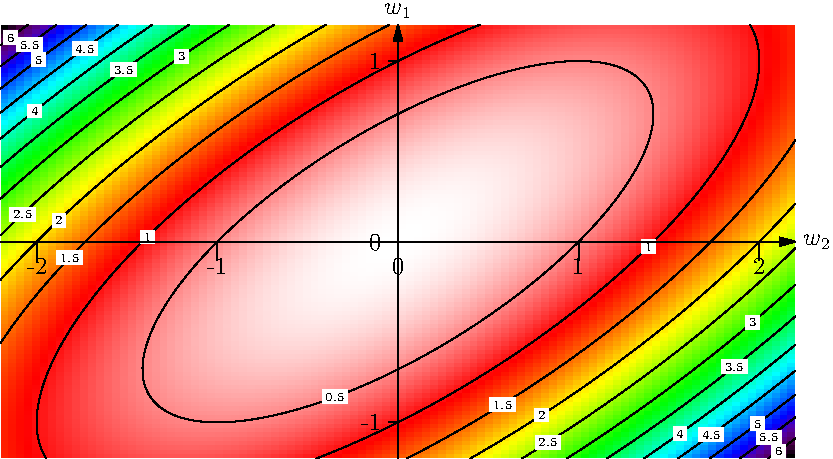
\includegraphics[width=.9\linewidth]{./figures/quadProblem.pdf}
\end{center}
\end{enumerate}
\end{document}
